This chapter will introduce the numerical framework implemented in \href{https://qojulia.github.io/WaveguideQED.jl/dev/}{WaveguideQED.jl}. The implementation is based on the time-binned continuous fockstate formalism introduced in Chapter 2. We show that it correctly recovers equations of motion in the limit of $\Delta t \rightarrow 0$ by doing a convergence study. Furthermore, we introduce Lazy Operator data structures, which are used in our software implementation to enhance performance.   

\section{Numerical Representation of One-photon States} \label{sec:onephoton_numerical}
In ch.~\ref{ch2}, we used the time-binned picture to derive the equations of motion for a single-photon scattering on a cavity. Ultimately, we took the limit of $\Delta t \rightarrow 0$ meaning infinitesimally small bins, thus restoring the continuous fockstate. In this section, however, we will keep the time-binned photon representation and show how we can obtain equivalent results numerically. 

If we consider a continuous photon state in $N$ bins with no more than a single photon, we will need a vector of size $N+1$ to represent it (plus one because we also need to represent vacuum $\ket{\emptyset}$). This is illustrated in Fig.~\ref{fig:onephoton_representation} with $N=5$. In this truncated Hilbert space, the effect of applying the operator $w_3^\dagger$ is then given as
\begin{equation}
    w_3^\dagger \ket{\psi} = \begin{pmatrix}
        0 & 0 & 0 & 0 & 0 & 0 \\
        0 & 0 & 0 & 0 & 0 & 0 \\
        0 & 0 & 0 & 0 & 0 & 0 \\
        1 & 0 & 0 & 0 & 0 & 0 \\
        0 & 0 & 0 & 0 & 0 & 0 \\
        0 & 0 & 0 & 0 & 0 & 0 \\
    \end{pmatrix} \cdot \begin{pmatrix}
        \textcolor{red}{\psi_\emptyset} \\
        \psi_1 \\
        \psi_2 \\
        \psi_3 \\
        \psi_4 \\
        \psi_5
    \end{pmatrix} = \begin{pmatrix}
        0 \\
        0 \\
        0 \\
        \textcolor{red}{\psi_\emptyset} \\
        0 \\
        0
    \label{eq:operator_matrix} \end{pmatrix} 
\end{equation}
here, $\psi_i$ denotes the value stored in element $i$ (starting from zero to represent vacuum and the subsequent $N$ elements to represent the single photon excitation). Figure \ref{fig:onephoton_representation} also shows the effect of applying the operator $w_3^\dagger$: Move the element in $\ket{\emptyset}$ to the element in time-bin $3$. In the sketch, we only denote non-zero changes with the arrow; therefore, it is understood that all other elements are zero after the operation. Note that Fig~\ref{fig:onephoton_representation} shows the physical effect of applying $w_3^\dagger$. Numerically, the result of applying such operations is, as we shall see, often stored in another vector \code{dpsi}, and a more accurate representation would therefore be to draw an arrow between the input vector \code{psi} and the vector that stores the resulting state \code{dpsi}. For the sake of simplicity, we omit this extra step in all illustrations.  
\begin{figure}[H]
    \centering
    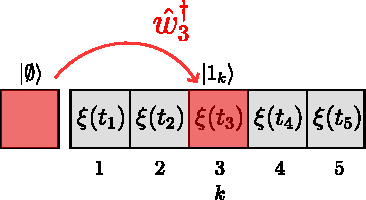
\includegraphics[width=0.5 \linewidth]{figures/one_photon_create.pdf}
    \caption{A numerical representation of the one-photon state and the effect of applying the creation operator $w_3^\dagger$. We only denote non-zero changes with the arrow; therefore, it is understood that all other elements are zero after the operation. Numerically, another vector \code{dpsi} would be used to store the result of the calculation. For simplicity, this vector is not shown either.}
    \label{fig:onephoton_representation}
\end{figure}
To solve the scattering problem, we combine the state of the waveguide with the state of the cavity by a tensor product. Since we only consider a total of one excitation, we can truncate the Hilbert space of the cavity to $\{ \ket{0},\ket{1} \}$ or equivalently a vector of length two. An arbitrary state of the waveguide and cavity can thus be described as:
\begin{equation}
    \ket{\psi} = \ket{0} \otimes \left( A_0 \ket{\emptyset}+ \sum_{k=1}^N \sqrt{\Delta t} \xi_0(t_k) \ket{1_k} \right ) + \ket{1} \otimes \left( A_1 \ket{\emptyset}+ \sum_{k=1}^N \sqrt{\Delta t} \xi_1(t_k) \ket{1_k} \right ) 
\end{equation}
where $A_0$, $A_1$, $\xi_0(t_k)$, $\xi_1(t_k)$ are the elements stored in a vector of the same structure as in Fig.~\ref{fig:onephoton_representation}. After the tensor product, we thus have a vector of length $2\cdot(N+1)$. We can here associate the first $N+1$ elements with the cavity being empty: $\ket{0}$ and the last $N+1$ with the cavity having one photon: $\ket{1}$. A numerical representation of this state can be seen in Fig.~\ref{fig:cavity_create}. The action of the operators $a^\dagger w_k$ and $a w_k^\dagger$ making up the interaction Hamiltonian in eq.~\eqref{eq:discretized_interaction} with $k = 3$ is also shown. Again, the interpretation is clear, $a^\dagger w_k$ removes an excitation from time-bin $k$ and places it in the cavity mode, while $a w_k^\dagger$ does the opposite. 


 
\begin{listing}[H]
\begin{minted}[
frame=lines,
framesep=2mm,
baselinestretch=1.2,
bgcolor=LightGray,
fontsize=\small,
linenos
]{julia}
function dpsi!(dpsi,psi,p,t)
    y,d,nsteps,dt = p
    timeindex = round(Int,t/dt,RoundDown) + 1
    dpsi .= 0
    dpsi[2+nsteps] = sqrt(y/dt)*psi[1+timeindex] - im*d*psi[2+nsteps]
    dpsi[1+timeindex] = -sqrt(y/dt)*psi[2+nsteps]
end
\end{minted}
\caption{Function to calculate the derivative, given by applying $- i H(t_k) = - i \delta_a a^\dagger a + \sqrt{\gamma/dt}(a^\dagger w_k - a w_k^\dagger)$ to the state {\fontfamily{pcr}\selectfont psi} and saved in {\fontfamily{pcr}\selectfont dpsi}.}
\label{ls:derivative}
\end{listing}
\begin{figure}
    \centering
    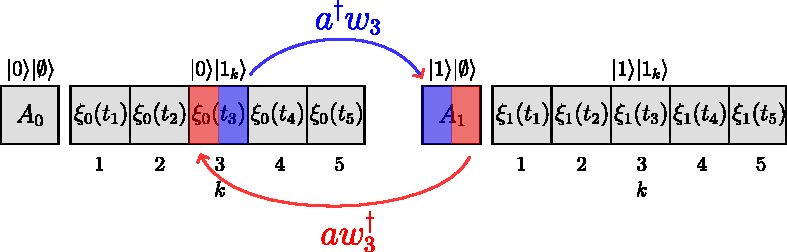
\includegraphics[width=0.8 \linewidth]{figures/cavity_destroy_create.pdf}
    \caption{A numerical representation of the combined state of a one photon state in the waveguide $\ket{1_k}$ and a cavity containing zero $\ket{0}$ or one photon $\ket{1}$. The effect of applying the operators $a^\dagger w_3$ and $a w_3^\dagger$ is also shown with blue and red arrows, respectively. }
    \label{fig:cavity_create}
\end{figure}

Based on these definitions of the operators, it is possible to set up a very simple simulation of the dynamics. The governing equation is Schr{\"o}dinger's equation $\frac{\partial}{\partial t} \ket{\psi} = - i H \ket{\psi}$, and in Code Sample \ref{ls:derivative} we implement a function in Julia that returns the derivate \code{dpsi} by applying $- i H(t_k) = - i \delta_a a^\dagger a + \sqrt{\gamma/dt}(a^\dagger w_k - a w_k^\dagger)$ to {\fontfamily{pcr}\selectfont psi} as depicted in Fig.~\ref{fig:onephoton_representation}. Notice that {\fontfamily{pcr}\selectfont timeindex} determines which bin the waveguide operators $w_k$ and $w_k^\dagger$ address. Line 5 updates $\ket{1}\ket{\emptyset}$ with $\sqrt{\gamma/\Delta t} a^\dagger w_k$ and $- i \delta_a a^\dagger a$. Line 6 updates $\ket{0}\ket{1_k}$ with $-\sqrt{\gamma/\Delta t} a w_k^\dagger$. This derivative function can then be passed to a differential equation solver to get the dynamics.

In the following, we consider a Gaussian input state with the wavefunction $\xi^{(1)}(t)$ defined as 
\begin{equation}
    \xi^{(1)}(t) = \sqrt{\frac{2}{\sigma}} \left(\frac{\log(2)}{\pi}\right)^{1/4} \exp\left(-\frac{2\log(2)(t-t_0)^2}{\sigma^2}\right) \label{eq:gaussian}
\end{equation}
In Code Sample \ref{ls:solver}, we use the derivative function from Code Sample \ref{ls:derivative} to solve the scattering of an input state with $\sigma = 1$ and $t_0 = 5$. We can compare the solution to the analytically obtainable solution to the equation of motion in eq.~\eqref{eq:single_EOM}. As shown in appendix \ref{app:analytical}, the analytical solution is given as:
\begin{equation}
    \xi^{(1)}_\mathrm{EOM}(t) =  \xi^{(1)}(t) - \sqrt{\gamma}\frac{\sqrt{\pi} e^{\frac{b^2}{4a}+bt_0}}{2\sqrt{a}}\left(\text{erf}\left(\frac{2a(t-t_0)-b}{2\sqrt{a}}\right) + \text{erf}\left(\frac{2at_0+b}{2\sqrt{a}}\right)\right) \label{eq:onephoton_analytical}
\end{equation}
with $a = 2 \log(2)/\sigma^2$ and $b = i \delta + \gamma/2$. The analytical solution is shown together with the numerical solution in Fig.~\ref{fig:singlephoton}. We see how the photon pulse is distorted from the interaction with the cavity. The dip in the scattered wavefunction around $t \approx 5.5/\gamma$ arises due to destructive interference between the reemitted field from the cavity and the reflected pulse. We will study this phenomenon in greater detail later. For now, it is important to notice the convergence in Fig.~\ref{fig:single_photon_convergence} showing that the two methods converge as the number of bins increases (meaning $\Delta t \rightarrow 0$). 

\begin{listing}[!ht]
\begin{minted}[
frame=lines,
framesep=2mm,
baselinestretch=1.2,
bgcolor=LightGray,
fontsize=\small,
linenos,
escapeinside=||,
mathescape=true
]{julia}
using DifferentialEquations
using LinearAlgebra
using PyPlot

#Define parameters
|$\gamma$|,|$\delta$|,dt = 1,0,0.1
times = 0:dt:10
N = length(times)
p = (|$\gamma$|,|$\delta$|,N,dt)

#Define input gaussian state with width s = 1 and arrival time t0=5
xi(t,s,t0) = sqrt(2/s)* (log(2)/pi)^(1/4)*exp(-2*log(2)*(t-t0)^2/s^2)
psi = zeros(ComplexF64,2*(N+1))
#Index 2:N+1 to adress $\ket{0}\ket{1_k}$ as in Fig. $\ref{fig:cavity_create}$
psi[2:N+1] .= sqrt(dt)*xi.(times,1,5)

#Define and solve ODE problem by giving initial state psi and differential operator dpsi!
prob = ODEProblem(dpsi!, psi, (times[1], times[end]+dt), p)
sol = solve(prob, OrdinaryDiffEq.DP5();reltol = 1.0e-8,abstol = 1.0e-10);
psi_out = sol[end][2:N+1]
\end{minted}
\caption{Code for solving scattering of single-photon pulse on onesided cavity. }
\label{ls:solver}
\end{listing}

\begin{figure}[H]
    \centering
    \subfloat[\label{fig:singlephoton}]{{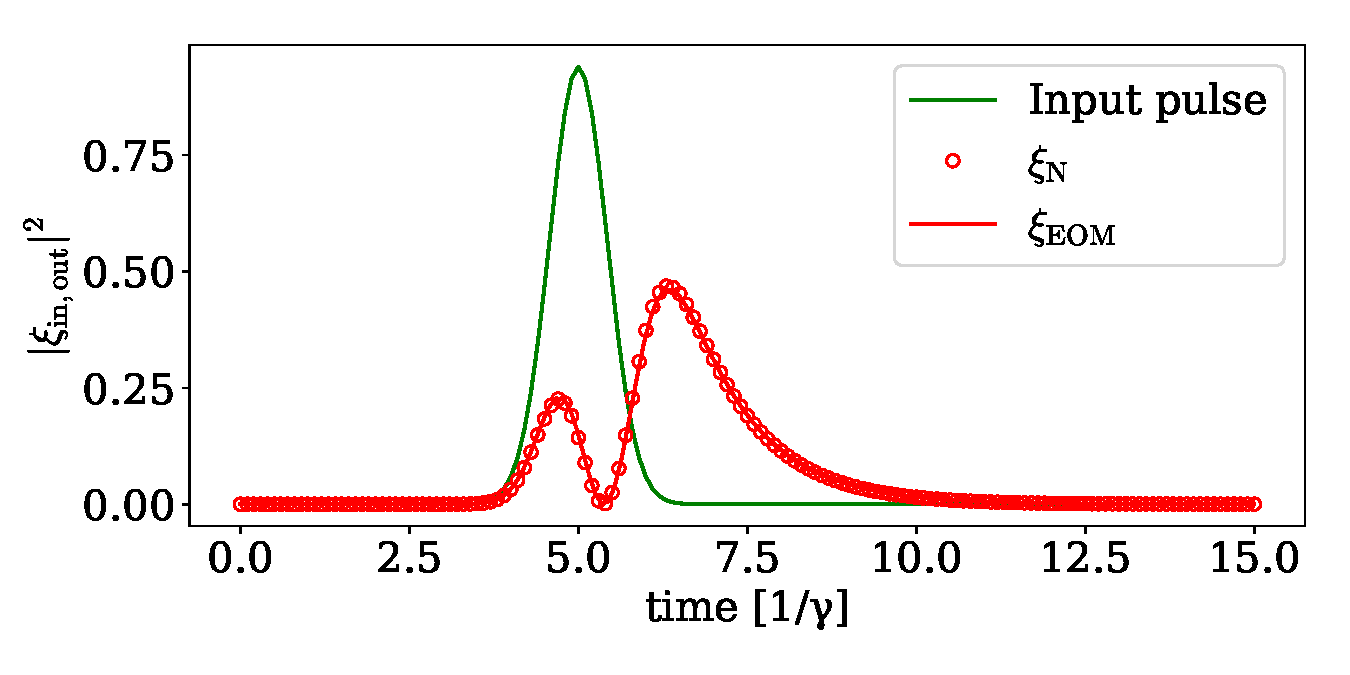
\includegraphics[width=0.49\textwidth]{figures/singlephoton.pdf}}}    \subfloat[\label{fig:single_photon_convergence}]{{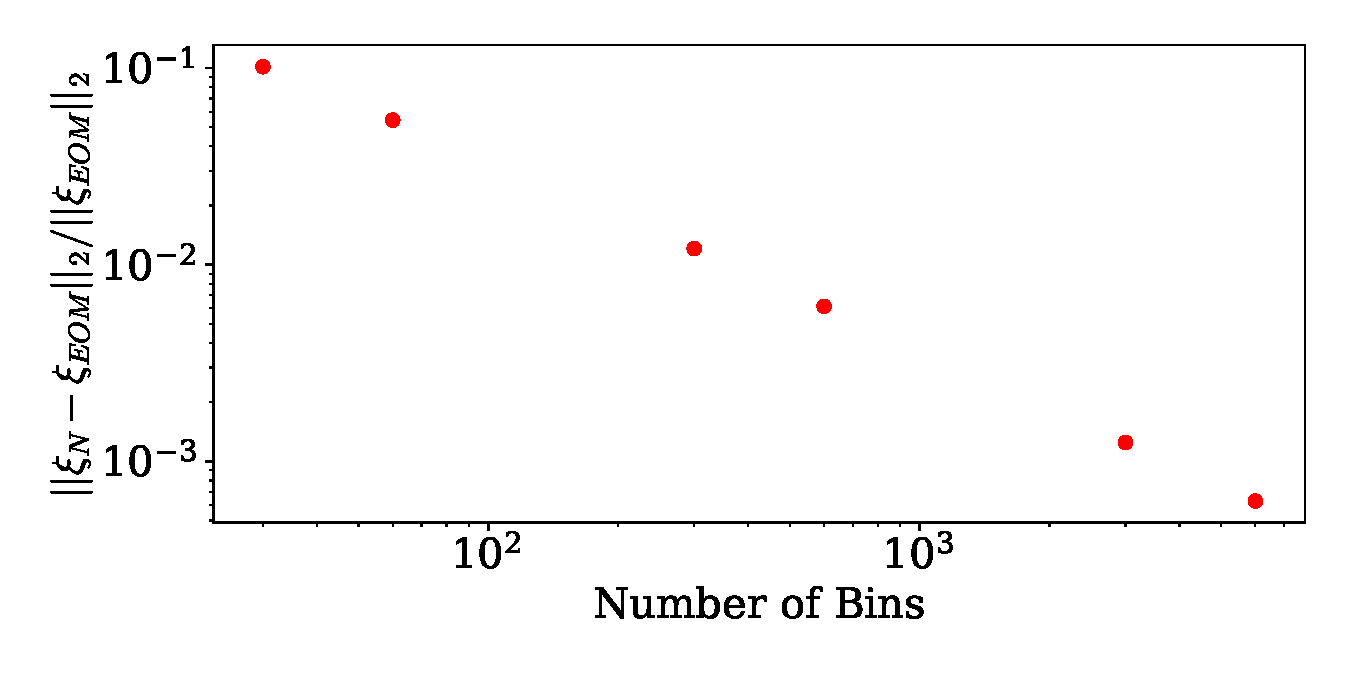
\includegraphics[width=0.49\textwidth]{figures/convergence.pdf} }}
    \caption{(a) The scattering of a Gaussian single-photon pulse defined in eq.~\eqref{eq:gaussian} on a single-sided cavity with $\sigma = 1$ and $t_0 = 5$. The solution to the equations of motion $\xi_\mathrm{EOM}$ from eq.~\eqref{eq:onephoton_analytical} is shown together with the numerical solution from the above code $\xi_\mathrm{N}$ (with a time-bin size of $\Delta t = 0.1/\gamma$). The two methods are seen to produce identical results. (b) Convergence plot showing the relative error in the L2-norm $||f||_2 = \int_{-\infty}^\infty |f(t)|^2 d t $ between the equation of motion solution and the numerical solution. }
\end{figure}

The above numerical implementation is very simple and fast, but it is also hardcoded to solve one specific problem. This is not the ultimate goal of the implementation, as we want it to be flexible and able to solve many different waveguide QED problems. The natural extension is to implement the operators $a$, $a^\dagger$, $w_k$, and $w_k^\dagger$ as matrices and then combine them through the tensor product $\otimes$. In the next section, we show how this can be done in 
\href{https://qojulia.org/}{QuantumOptics.jl} a package for simulating Quantum Optics in Julia \cite{Kramer2018QuantumOptics.jl:Systems}.

\section{Sparse Operators \label{sec:sparseoperators}}
In this section, we show how to implement the waveguide operators $w_k$ and $w_k^\dagger$ as sparse matrices in \href{https://qojulia.org/}{QuantumOptics.jl}. As we shall see the cost of allocating memory for these matrices quickly becomes a limiting factor as the size of the problem grows. Lazy operators, introduced in section \ref{sec:lazyoperators} is the solution. For now, it is, however, still instructive to consider the more straightforward case of sparse matrices. 

In the truncated Hilbert space of only a single-photon time-binned state, we can define waveguide operators according to the transition they represent $w_k = \ket{\emptyset} \bra{1_k}$ and $w_k^\dagger = \ket{1_k} \bra{\emptyset}$. In Julia, using \href{https://qojulia.org/}{QuantumOptics.jl}, this can be accomplished by the code in Code Sample \ref{ls:sparseoperators}. Here, we define the basis of the waveguide \code{bw} as a GenericBasis, which is an object subsequently used to define kets belonging to that Hilbert space. In this case, the most important property of the Basis is that it contains the size of Hilbert space ($N+1$, where $N$ is the number of bins). $w_k$ is then initialized by taking the tensor product between the ket $\ket{\emptyset}$ and bra $\bra{1_k}$. $\ket{\emptyset}$ is defined from {\fontfamily{pcr}\selectfont basisstate(bw,1)}: A state belonging to the basis of waveguide {\fontfamily{pcr}\selectfont bw}, with the first element being occupied. Similarly,  $\bra{1_k}$ is then {\fontfamily{pcr}\selectfont dagger(basisstate(bw,1+timeindex))}, where {\fontfamily{pcr}\selectfont timeindex} here controls the time-bin we are addressing (in this case bin number one) and \code{dagger()} turns the ket into a bra. $w_k^\dagger$ is also just defined from applying \code{dagger()} to \code{w}.
\begin{listing}[H]
\begin{minted}[
frame=lines,
framesep=2mm,
baselinestretch=1.2,
bgcolor=LightGray,
fontsize=\small,
linenos,
escapeinside=||,
mathescape=true
]{julia}
dt = 0.1
times = 0:dt:10
N = length(times)
bw = GenericBasis(N+1)
timeindex = 1
w = basisstate(bw,1) |$\otimes$| dagger(basisstate(bw,1+timeindex))
wd = dagger(w)
\end{minted}
\caption{Code for creating waveguide operators $w$ and $w^\dagger$ as sparse matrices.}
\label{ls:sparseoperators}
\end{listing}
With the operators defined, we can combine them with a cavity through the tensor product $\otimes$ (in Julia: $\backslash \mathrm{otimes}$ followed by TAB). In Code Sample \ref{ls:combine}, we define the basis of the cavity \code{bc} containing at max one photon, the annihilation operator of this basis \code{a = destroy(bw)} and creation operator \code{ad = create(bw)}. These are then combined with the waveguide operators \code{w} and \code{wd} via tensor products to form $a^\dagger w_k$ and $a^\dagger w_k$, which finally can be combined to form the Hamiltonian $H = i \hbar \sqrt{\gamma/\Delta t}(a^\dagger w_k - a w_k^\dagger) +  \hbar \delta a^\dagger a$. Note that in all code and simulations, we set $\hbar = 1$.

\begin{listing}[H]
\begin{minted}[
frame=lines,
framesep=2mm,
baselinestretch=1.2,
bgcolor=LightGray,
fontsize=\small,
linenos,
escapeinside=||,
mathescape=true
]{julia}
bc = FockBasis(1)
a = destroy(bw)
ad = create(bw)
n = (ad*a) |$\otimes$| identityoperator(bw)
adw = ad |$\otimes$| w
wda = a |$\otimes$| wd
H = im*sqrt(|$\gamma$| / dt) *(adw - wda) + |$\delta$| * n 
\end{minted}
\caption{Code for combining cavity annihilation and creation operators $a$ and $a^\dagger$ with waveguide operators $w$ and $w^\dagger$.}
\label{ls:combine}
\end{listing}

In Code Sample \ref{ls:combine}, we, however, only created the Hamiltonian for the first timestep. Our Hamiltonian changes at each timestep, so we need to define a time-dependent problem. This is done in Code Sample \ref{ls:timedependent}, where we calculate the Hamiltonian for all timesteps in lines 1-8 and define a function that returns the Hamiltonian for the corresponding timestep in lines 9-12. In lines 14-16, we define the input state, in a similar fashion as in the previous section, except that we can now just combine the cavity and waveguide through the tensor product. Finally, say we are interested in the number of photons inside the cavity as a function of time, we can define the expectation-value function \code{na} in line 18. In line 19, we then solve the time-dependent problem by using our defined input state \code{psi\_in}, our function that returns our time-dependent Hamiltonian \code{Htime}, and our expectation value function \code{na}.

\begin{listing}[H]
\begin{minted}[
frame=lines,
framesep=2mm,
baselinestretch=1.2,
bgcolor=LightGray,
fontsize=\small,
linenos,
escapeinside=||,
mathescape=true
]{julia}
Hlist = Array{Operator}(undef,N)
for i in 1:N
    w = basisstate(bw,1) |$\otimes$| dagger(basisstate(bw,1+i))
    wd = dagger(w)
    adw = ad |$\otimes$| w
    wda = a |$\otimes$| wd
    Hlist[i] = im*sqrt(|$\gamma$| / dt) *(adw - wda) + |$\delta$|*n
end
function Htime(time,psi)
    timeindex = round(Int,time/dt,RoundDown)+1
    Hlist[timeindex]   
end

psi_waveguide = Ket(bw)
psi_waveguide.data[2:N+1] .=  sqrt(dt)*xi.(times,1,5)
psi_in = fockstate(bc,0) |$\otimes$| psi_waveguide

na(time,psi) = expect(n,psi)
_,n = timeevolution.schroedinger_dynamic(times, psi_in, Htime,fout=na)
\end{minted}
\caption{Code for defining a time-dependent problem in Julia.}
\label{ls:timedependent}
\end{listing}

In Fig.~\ref{fig:cavity_occupation}, we show the population in the cavity as a function of time for different detuning values $\delta$ as calculated by Code Sample \ref{ls:timedependent}. It is clear that as the detuning increases, the pulse absorption decreases. Comparing with Fig.~\ref{fig:singlephoton_wf}, where we show output wavefunction $\xi_{out}(t)$, we see that for larger detuning no dip appears. This is due to the lower cavity population, meaning less destructive interference and thus less distortion of the photon wavepacket. 

\begin{figure}[H]
    \centering
    \subfloat[\label{fig:cavity_occupation}]{{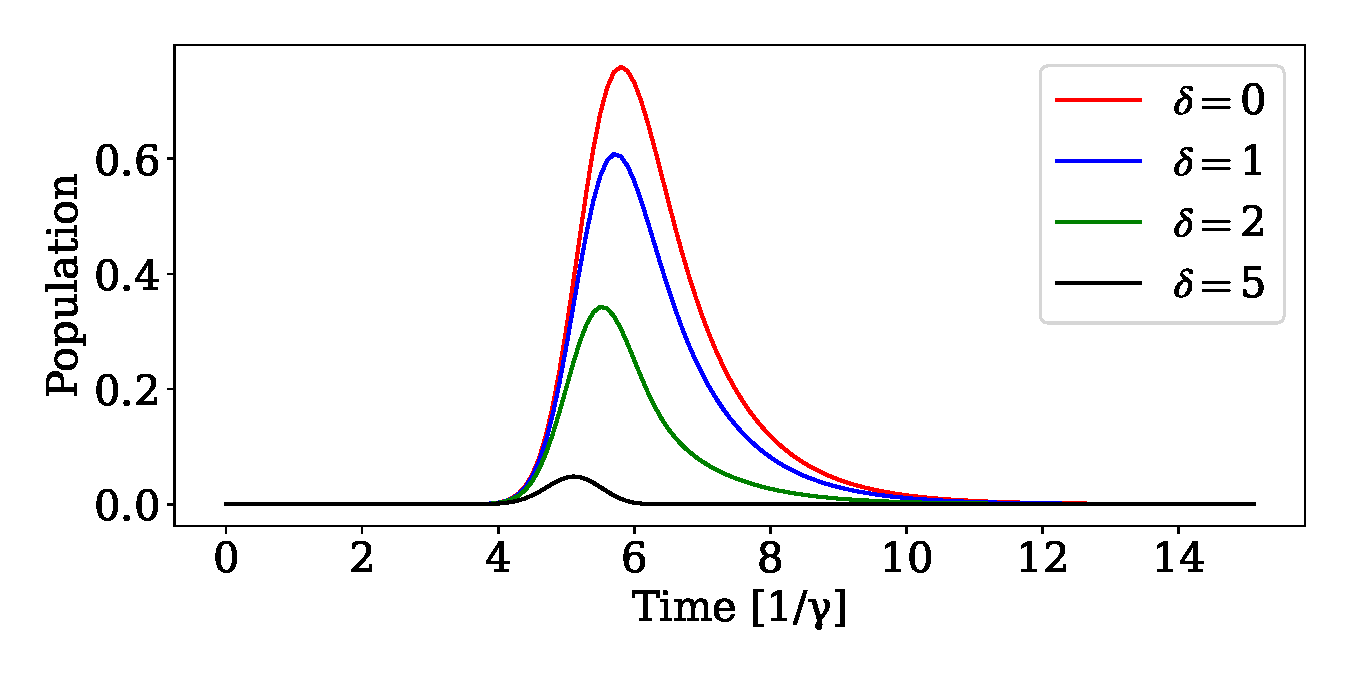
\includegraphics[width=0.49\textwidth]{figures/photon_number.pdf}}}    \subfloat[\label{fig:singlephoton_wf}]{{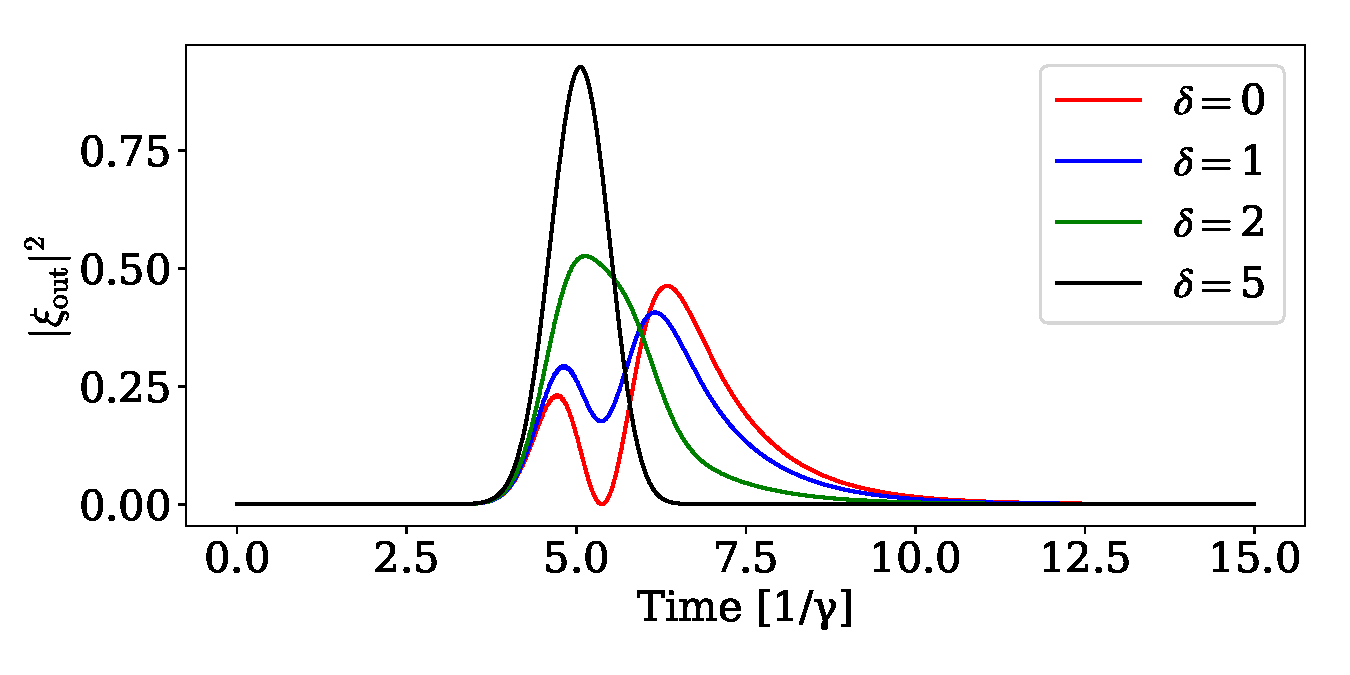
\includegraphics[width=0.49\textwidth]{figures/singlephoton_wavefunction.pdf} }}
    \caption{(a) Cavity photon population as a function of time for different values of detuning. (b) The scattered wavefunction as a function of time.}
\end{figure}


In this example, representing the operators $w_k$ and $w_k^\dagger$ as sparse matrices worked well since the Hilbert spaces we considered were small. In the next section, we will consider two-photon states, and as we shall see, the overhead associated with allocating these matrices quickly dominates the performance. 


\section{Numerical Representation of Two-photon States \label{sec:twophoton_numerical}}
As shown in chapter \ref{ch2}, the two-photon time binned state is given as:
\begin{equation}
    \ket{\psi} = \sqrt{2} \sum_{i=1}^N \sum_{k > i}^N \Delta t \xi_2\left (t_i,t_k\right ) \mid 1_{t_i} 1_{t_k}\rangle + \sum_{i=1}^N \Delta t \xi_2\left (t_i,t_i\right )\left|2 t_i\right\rangle
\end{equation}
Numerically, we need $N(N-1)/2 + N = N(N+1)/2$ bins to represent this state, where $N$ here is the number of bins of the single-photon state. The two-photon state is numerically a vector with $N(N+1)/2$ elements but is best visualized as a matrix, as shown in Fig.\ \ref{fig:twophoton_representation}. Note that the lower triangular part is not stored in memory due to the symmetry of the two-photon state. In the Figure, we also show how the creation operator $w_3^\dagger$ relates a one-photon state to a two-photon state, where the darker red square carries a factor of $\sqrt{2}$ since $w_3^\dagger \ket{1_3} = \sqrt{2}\ket{2_3}$. Here we imagine that we have a combined state of a single-photon state and a two-photon state, where the first element is the vacuum, the following $N$ elements are the single-photon state, and the last $N(N+1)/2$ elements are the two-photon state. In this truncated space, we can thus also write the creation operator as:
\begin{equation}
    w_k^\dagger = \ket{1_k} \bra{\emptyset} + \sum_{j < k} \ket{1_k,1_j} \bra{1_j} + \sum_{j > k} \ket{1_j,1_k} \bra{1_j} + \sqrt{2} \ket{2_k} \bra{1_k} 
\end{equation}
where the first term takes the vacuum to a single-photon state (as introduced earlier in sec.~\ref{sec:sparseoperators}), the second term takes a single-photon state at a previous time $j$ to a combined state of a photon at time $j$ and $k$, and the third term is similar and takes a future single-photon state at time $j$ and takes it into the combined state of a photon at time $j$ and $k$. The last term takes the single-photon at exactly time $k$ into the state with two photons in the same time bin $k$ and, thus, carries a factor of $\sqrt{2}$. 

\begin{figure}[H]
    \centering
    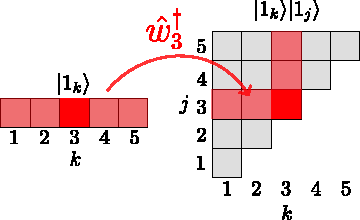
\includegraphics[width=0.6 \linewidth]{figures/twophoton.pdf}
    \caption{Numerical representation of a two-photon state together with the action of the waveguide operator $w_3^\dagger$ on a single-photon state. The darker red square has a factor of $\sqrt{2}$ to satisfy $w_3^\dagger \ket{1_3} = \sqrt{2} \ket{2_3}$ }
    \label{fig:twophoton_representation}
\end{figure}


Again this can be described as a sparse matrix. However, the sparse matrix is now of size $1+N+N(N+1)/2$. With $N=100$, this corresponds to a $5151 \mathrm{x} 5151$ matrix. If we now want to combine it with a cavity containing two photons to construct the operators $a^\dagger w_k$ and $a w_k^\dagger$, we have a tensor product between a $3\mathrm{x}3$ matrix and a $5151\mathrm{x}5151$ matrix. As shown in section \ref{sec:sparseoperators}, we construct and perform this tensor product for each timestep in the simulation. A quick benchmark reveals that this task quickly grows expensive. In Fig.~\ref{fig:createoperator_bench}, we compare the time spent creating the Hamiltonians and the time spent solving the actual differential equations. As the number of bins increases, we see that we spend most of the time just creating the Hamiltonian for the problem. The way the Hamiltonian change is, however, well known. We can exploit this and implement the operator instead as an object that executes a predefined function dependent on time, which mimics the behavior of doing the matrix multiplication. This is the core principle behind the Lazy Operators used in WaveguideQED.jl, which we will introduce in the next section. 


\begin{figure}[H]
    \centering
    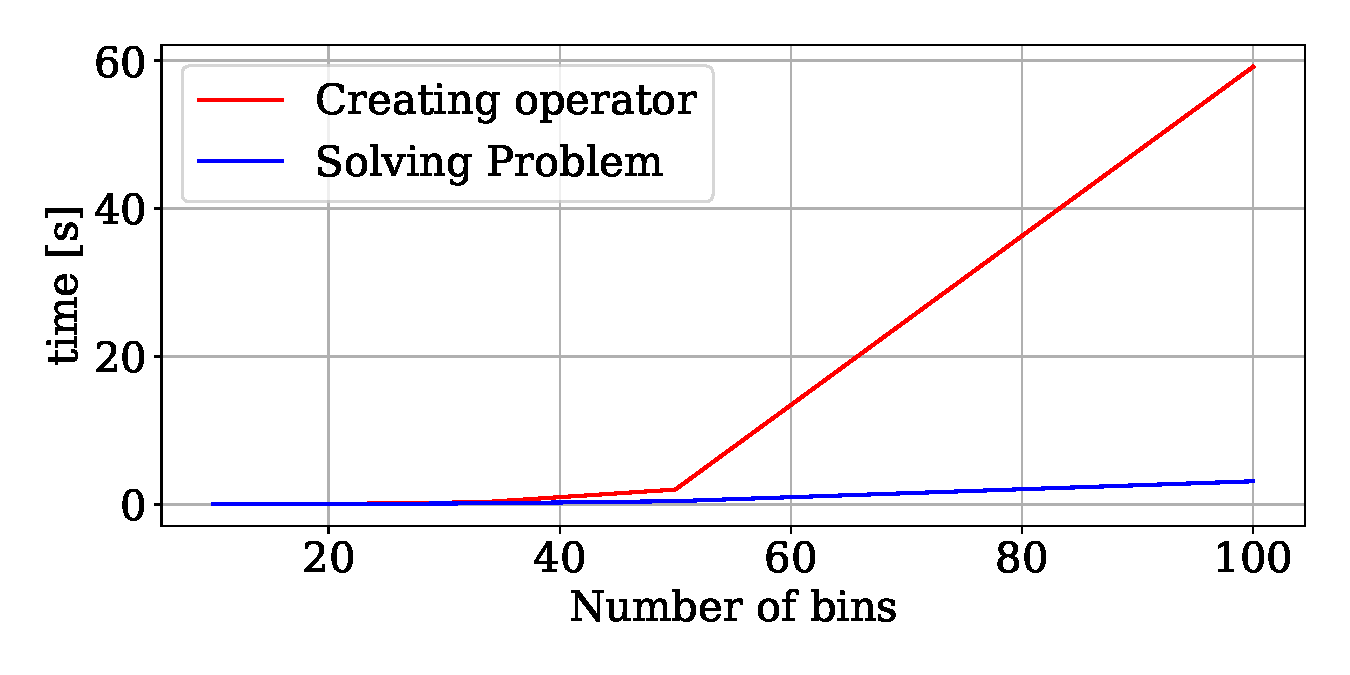
\includegraphics[width = 0.6 \linewidth]{figures/allocatingvssolving_bench.pdf}
    \caption{Comparison between time spend creating the Hamiltonians and solving the actual problem (here scattering of a two-photon pulse of a cavity with the Hamiltonian defined in eq.~\eqref{eq:discretized_interaction} ). It is evident that for more than $N\approx 60$, the majority of the computational time is taken up by just creating the Hamiltonians.}
    \label{fig:createoperator_bench}
\end{figure}


\section{Lazy Operators\label{sec:lazyoperators}}
Motivated by the significant overhead in creating the Hamiltonian for each time step, as seen in section \ref{sec:twophoton_numerical}, we want to represent the waveguide operator $w_k^\dagger$ as an object that can be applied to a ket and perform the already known operation. If we only consider a waveguide ket, the implementation is simple. In Code Sample \ref{ls:lazyoperator}, we define a structure representing the waveguide operator $w_k^\dagger$. \code{basis\_l} and \code{basis\_r} are objects that contain information about the Hilbert space and will become important when we later want to combine the structure with operators belonging to other Hilbert spaces. \code{factor} allows us to define arithmetic operations. As an example, $\beta * w_k^\dagger$, would update factor as: \code{factor = $\beta$ * factor}. Finally, \code{timeindex} allows us to change $k$ in each timestep. In the first timestep, we want to apply the operator $w_1^\dagger$, and we thus set \code{timeindex = 1}. In the next timestep, we then update \code{timeindex = 2} and so on.

\begin{listing}[H]
\begin{minted}[
frame=lines,
framesep=2mm,
baselinestretch=1.2,
bgcolor=LightGray,
fontsize=\small,
linenos,
escapeinside=||,
mathescape=true
]{julia}
abstract type WaveguideOperator{B1,B2} <: AbstractOperator{B1,B2} end
mutable struct WaveguideCreate{B1,B2,Np,idx} <: WaveguideOperator{B1,B2}
    basis_l::B1
    basis_r::B2
    factor::ComplexF64
    timeindex::Int
end
\end{minted}
\caption{Structure in Julia for defining Lazy Operator.}
\label{ls:lazyoperator}
\end{listing}

But how is the multiplication done? In Code Sample \ref{ls:multiplcation_code} lines 1-5, we show the multiplication routine for $w_k^\dagger$ on a state that contains a single photon. The routine updates the vector result as: \code{result = factor * $\alpha$ * $w_k^\dagger$ * b +  $\beta$ * result} (note the presence of \code{factor}). The routine for doing two-photon multiplication is more complex and can be viewed in appendix \ref{app:twophotonroutine}. In lines 6-10, the multiplication symbol "*" is overloaded, and in lines 11-15, we apply the operator $w_k^\dagger$ to a vacuum state $\ket{\emptyset}$. Note that we have created a custom basis \code{WaveguideBasis} from which we can initialize our operator with \code{destroy(bw)} and a state belonging to this Hilbert space with \code{Ket(bw)}. The resulting waveguide state \code{result} = $w_k^\dagger \ket{\emptyset}$, is shown in Fig.~\ref{fig:creationoperator} for different $k$'s. As expected, we see sharp spikes at the defined $k$'s.  
\begin{listing}[H]
\begin{minted}[
frame=lines,
framesep=2mm,
baselinestretch=1.2,
bgcolor=LightGray,
fontsize=\small,
linenos,
escapeinside=||,
mathescape=true
]{julia}
function mul!(result,a::WaveguideCreate{B,B,1,idx},b,alpha,beta) where {B,idx}
    rmul!(result,beta)
    result[1] += alpha*a.factor*b[a.timeindex+1]
    result
end
function *(op::AbstractOperator{BL,BR}, psi::Ket{BR,T}) where {BL,BR,T}
    result = Ket{BL,T}(op.basis_l,similar(psi.data,length(op.basis_l)))
    mul!(result,op,psi)
    return result
end
bw = WaveguideBasis(1,times)
wd = create(bw)
wd.timeindex = k
psi = Ket(bw)
psi.data[1] = 1
result = wd*psi
\end{minted}
\caption{Code for multiplication with Lazy waveguide operator. Lines 1-5 show how we can perform the action of the operation by the matrix in eq.~\eqref{eq:operator_matrix} and illustrated in Fig.~\ref{fig:onephoton_representation}. Lines 6-10 show how the multiplication is performed ad lines 11-16 we create the operator and perform the operation. }
\label{ls:multiplcation_code}
\end{listing}


\begin{figure}
    \centering
    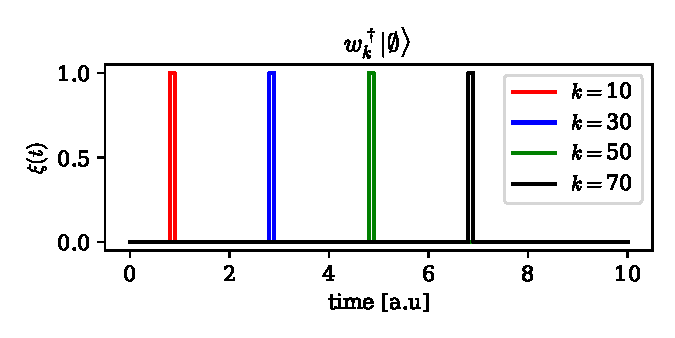
\includegraphics[width=0.6\linewidth]{figures/creationoperation.pdf}
    \caption{The one-photon wavefunction $\xi^{(1)}(t)$ as a function of time for the state $w_k^\dagger \ket{\emptyset} = \sum_i \xi(t_i) \ket{1_i}$ with $\xi(t_i) = \delta_{i,k}$ for different $k$'s. }
    \label{fig:creationoperator}
\end{figure}


Let us consider if we want to add two waveguide operators. If they were matrices, we could just add the elements together, but this is not possible with the LazyOperator implementation. Instead, we create another LazyOperator object \code{LazySum}, representing the sum of operators. The structure of the \code{LazySum} can be seen in 
Code Sample \ref{ls:lazysum}. Lines 1-6 define the structure, where \code{factors} are for arithmetic operations, and \code{operators} is a vector or tuple containing the operators to be summed. Lines 7-12 define how LazySum objects are added together; the fields \code{factors} and \code{operators} are concatenated, and a new LazySum object is instantiated. Lines 13-19 define the multiplication routine, where we loop over all operators in the \code{operators} field. Adding two waveguide operators can thus just be defined as creating a \code{LazySum} object as shown in Code Sample \ref{ls:additionwaveguide}.

\begin{listing}[H]
\begin{minted}[
frame=lines,
framesep=2mm,
baselinestretch=1.2,
bgcolor=LightGray,
fontsize=\small,
linenos,
escapeinside=||,
mathescape=true
]{julia}
mutable struct LazySum{BL,BR,F,T} <: AbstractOperator{BL,BR}
    basis_l::BL
    basis_r::BR
    factors::F
    operators::T
end
function +(a::LazySum{B1,B2}, b::LazySum{B1,B2}) where {B1,B2}
    check_samebases(a,b)
    factors = _cat(a.factors, b.factors)
    ops = _cat(a.operators, b.operators)
    @samebases LazySum(a.basis_l, a.basis_r, factors, ops)
end
function mul!(result::Ket{B1},a::LazySum{B1,B2},b::Ket{B2},alpha,beta) where {B1,B2}
    mul!(result,a.operators[1],b,alpha*a.factors[1],beta)
    for i=2:length(a.operators)
        mul!(result,a.operators[i],b,alpha*a.factors[i],1)
    end
    return result
end
\end{minted}
\caption{LazySum implementation. Lines 1-6 define the structure. Lines 7-12 define how LazySum objects are added together. Lines 13-19 define the multiplication operation.}
\label{ls:lazysum}
\end{listing}

\begin{listing}[H]
\begin{minted}[
frame=lines,
framesep=2mm,
baselinestretch=1.2,
bgcolor=LightGray,
fontsize=\small,
linenos,
escapeinside=||,
mathescape=true
]{julia}
function +(a::WaveguideOperator,b::WaveguideOperator)
    @assert a.basis_l == b.basis_l
    @assert a.basis_r == b.basis_r
    LazySum(a) + LazySum(b)
end
two_wd = wd + wd #LazySum
\end{minted}
\caption{Addition of waveguide operators returning a LazySum. }
\label{ls:additionwaveguide}
\end{listing}

In all of the above, we assumed that we were only considering the Hilbert space waveguide. However, we want to combine the waveguide operator with other quantum systems through the tensor product. Naturally, we, therefore, need to introduce a LazyTensor object. The code for performing the lazy tensor product is much more complicated than the lazy sum case. Thus, instead of going over the code in its entirety, we instead consider a specific example and illustrate how we can perform a lazy tensor operation. Let us consider a tensor product between two two-level systems. We can write this as:
\begin{equation}
    \left (a\ket{g}+b\ket{e} \right ) \otimes \left(c\ket{g}+d\ket{e} \right) =  \begin{pmatrix} {a} \\ {b} \end{pmatrix} \otimes \begin{pmatrix} {c} \\ {d} \end{pmatrix} = \begin{pmatrix} {a}{c} \\ {a} {d} \\ {b}{c} \\ {b}{d} \end{pmatrix}
\end{equation}
The transition operator for excited to ground state is $\sigma = \ket{g}\bra{e} = \begin{pmatrix}
    0 & 0 \\ 1 & 0
\end{pmatrix}$ and if we want to apply it to the second emitter, we tensor it with the identity operator. Without inferring the tensor product lazily, this would look like:
\begin{equation}
     I \otimes \sigma  \begin{pmatrix} {a}{c} \\ {a}{d} \\ {b}{c} \\ {b}{d} \end{pmatrix} =  \begin{pmatrix}
    1 & 0 \\ 0 & 1
\end{pmatrix} \otimes \begin{pmatrix}
    0 & 1 \\ 0 & 0
\end{pmatrix} \begin{pmatrix} {a}{c} \\ {a}{d} \\ {b}{c} \\ {b}{d} \end{pmatrix} = \begin{pmatrix}
0 & 1 & 0 & 0 \\
0 & 0 & 0 & 0 \\
0 & 0 & 0 & 1 \\
0 & 0 & 0 & 0
\end{pmatrix} \begin{pmatrix} {a}{c} \\ {a}{d} \\ {b}{c} \\ {b}{d} \end{pmatrix} = \begin{pmatrix} {a}{d} \\ 0 \\ bd \\ 0 \end{pmatrix}
\end{equation}

This operation could, however, also have been done by first applying $\sigma$ to the first two elements (notice we don't need to subsequently apply the identity operator):
\begin{equation}
    I \otimes \sigma \begin{pmatrix} {a}{c} \\ {a}{d} \\ {b}{c} \\ {b}{d} \end{pmatrix} = \begin{pmatrix}
    \color{red}{\begin{pmatrix}
    0 & 1 \\ 0 & 0
\end{pmatrix}} \\ \color{blue}{\begin{pmatrix}
    0 & 1 \\ 0 & 0
\end{pmatrix}}
\end{pmatrix} \begin{pmatrix} \color{red}{a}{c} \\ \color{red}{a}{d} \\ \color{blue}{b}{c} \\ \color{blue}{b}{d} \end{pmatrix} = \begin{pmatrix} \color{red}{a}{d} \\ 0 \\ \color{blue}{bd} \\ 0 \end{pmatrix}
\end{equation}
where it is here understood that the red matrix is applied to red elements and the blue matrix to blue elements. If we instead wanted to apply $\sigma \otimes I$, this would look like: 
\begin{equation}
    \sigma \otimes I \begin{pmatrix} {a}{c} \\ {a}{d} \\ {b}{c} \\ {b}{d} \end{pmatrix} = \begin{pmatrix}
    \color{red}{\begin{pmatrix}
    0 & 1 \\ 0 & 0
\end{pmatrix}} \\ \color{blue}{\begin{pmatrix}
    0 & 1 \\ 0 & 0
\end{pmatrix}}
\end{pmatrix} \begin{pmatrix} \color{red}{a}{c} \\ \color{blue}{a}{d} \\ \color{red}{b}{c} \\ \color{blue}{b}{d} \end{pmatrix} = \begin{pmatrix} \color{red}{b}{c} \\  \color{blue}{b}{d}  \\ 0 \\ 0 \end{pmatrix}
\end{equation}
We are now applying the matrices on a smaller vector formed by taking every second element. The formula for the index $\mathrm{I}$ of element $i$ in system 1 and element $j$ in system 2 is: $\mathrm{I} = i + 2\cdot(j-1)$. More generally, if we have multiple systems, we can access any arbitrary element by calculating the index as shown in Code Sample \ref{ls:lazy_index}:
\begin{listing}[H]
\begin{minted}[
frame=lines,
framesep=2mm,
baselinestretch=1.2,
bgcolor=LightGray,
fontsize=\small,
linenos,
escapeinside=||,
mathescape=true
]{julia}
I = indices[1]
for k in 2:length(indices)
    I += strides[k]*(indices[k]-1)
end
\end{minted}
\caption{Calculates the index \code{I} to access element \{i,j,k,...\} given by the vector \code{indices}. \code{Strides} is a vector containing strides for each sub-Hilbert space and is calculated in Code Sample \ref{ls:lazy_stride} }
\label{ls:lazy_index}
\end{listing}
where \code{indices} is a vector containing the indices of the elements that we want to access such that the first element $i$ is the index of the element in subsystem 1, the second element $j$ is the index of the element in subsystem 2, and so forth. \code{strides} is a vector containing the strides of the basis and can be calculated as shown in Code Sample \ref{ls:lazy_stride}:
\begin{listing}[H]
\begin{minted}[
frame=lines,
framesep=2mm,
baselinestretch=1.2,
bgcolor=LightGray,
fontsize=\small,
linenos,
escapeinside=||,
mathescape=true
]{julia}
strides[1] = 1
for m=2:length(shape)
    strides[m] = strides[m-1]*shape[m-1]
end
\end{minted}
\caption{Calculates the stride of each sub-Hilbert space, here \code{shape} is the sizes of the sub-Hilbert spaces. }
\label{ls:lazy_stride}
\end{listing}
where \code{shape} is the sizes of the subsystems. In the above case \code{shape = (2,2)} and \code{strides = (1,2)}. Using these indices, we can infer how the operators should be applied. The actual code for performing the LazyTensor product is a bit more involved but uses this principle. A Code Sample can be seen in appendix \ref{app:lazytensor}.

With the LazyOperators implemented, we are now ready to solve a two-photon pulse scattering on a cavity. In Fig.~\ref{fig:lazybench}, we benchmark the LazyOperator implementation vs. the Sparse operator implementation. The performance gain is huge for more than $\approx 50$ bins. Note that the time for the LazyOperator benchmark is both creating the operators and solving the problem. There is some small constant overhead related to creating the LazyOperators, which for small numbers of bins, makes it slightly slower than the sparse method. However, the time-bin picture is barely valid for this number of bins. In any realistic simulation, more than $100$ bins are used, and the performance gain is significant. The performance gain comes from not having to allocate the matrices and also because we are no longer looping through a sparse matrix where looking up indices is slow.     

\begin{figure}[H]
    \centering
    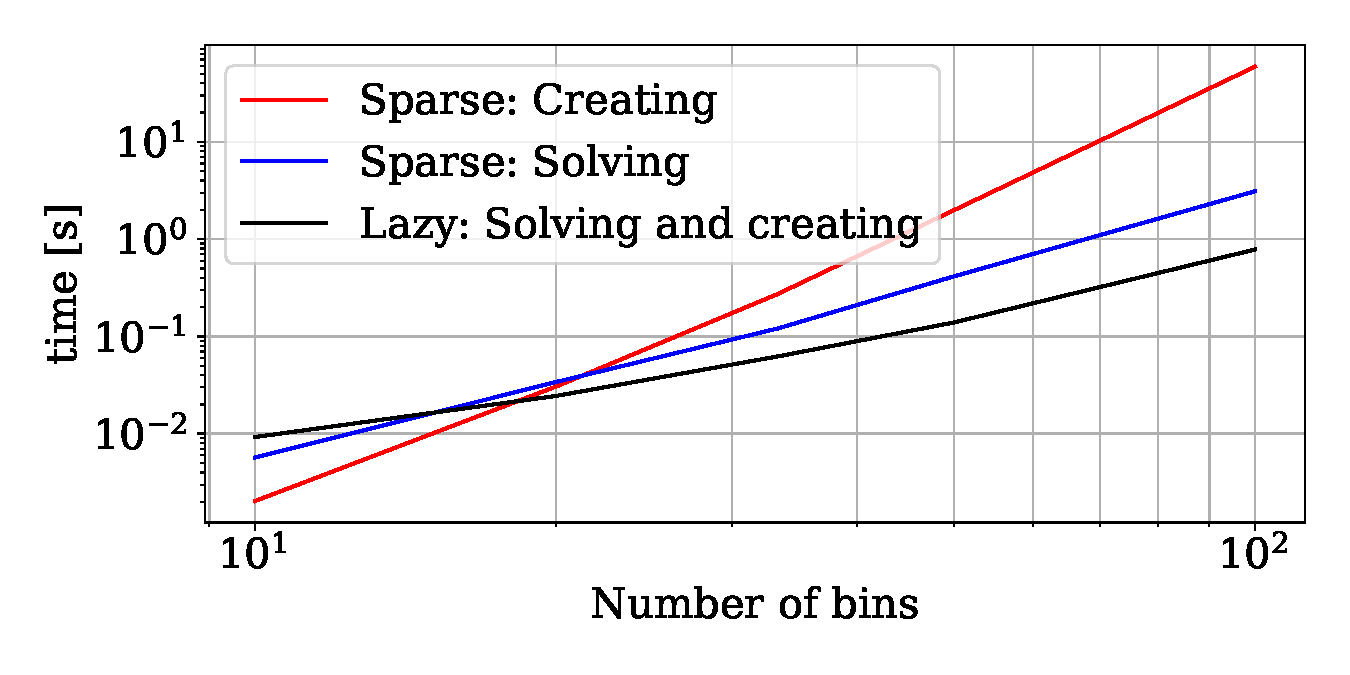
\includegraphics[width=0.6\linewidth]{figures/lazy_bench.pdf}
    \caption{Benchmark of lazy operator implementation compared to the time taken to create Hamiltonians in sparse version, and time taken to solve the problem in sparse version. We see that the time taken to solve the problems is almost equivalent, meaning that there is effectively no overhead in creating the Lazy operators.}
    \label{fig:lazybench}
\end{figure}


\section{Twophoton Scattering: Cavity vs. Emitter \label{sec:twophoton_emitter_vs_cavity}}
One of the major advantages of the numerical implementation in WaveguideQED.jl is flexibility. In this section, we will illustrate the flexibility by considering the scattering of a two-photon pulse on a cavity and emitter, respectively. In sec.~\ref{sec:twophoton_continuous}, we derived the equations of motion for a two-photon pulse scattering on a cavity, and we can use these to confirm that our implementation is also working for two-photon states. For the scattering of an emitter, even though it is mathematically close to the cavity (we just restrict the total number of photons to one), we would have to rederive the equations of motion as this introduces non-trivial effects, such as stimulated emission. In the numerical framework, it is trivial to change the operator $a \rightarrow \sigma$ thus showcasing its strength.


 We start by considering the scattering of a two-photon pulse in Fig.~\ref{fig:twophoton_detuning}. The code for setting this up in WaveguideQED.jl is shown in Code Sample \ref{ls:twophoton_scattering}, and a convergence study using the hierarchical differential equations in eq.~\eqref{eq:twophotonEOM} is done in appendix \ref{app:twophoton_convergence}. Note that the waveguide operators \code{w} and \code{wd} in Code Sample \ref{ls:twophoton_scattering} are effortlessly combined with operators from QuantumOptics.jl. Behind the scenes, lazy operations such as LazyTensor, LazySum, and LazyProduct, are all performed such that the user can manipulate the operators with $\otimes$,$+$,$-$, and $*$ as if they were standard operators defined via matrices. This allows for flexibility in setting up simulations and gives an intuitive user interface. 
 
 The initial state here consists of two one-photon Gaussian pulses $\ket{\psi}_{in} = \sum_k \sum_j \xi^{(2)}(t,t') \Delta t w_k^\dagger w_j^\dagger \ket{\emptyset}$ with $\xi^{(2)}(t,t') = \xi^{(1)}(t) \xi^{(1)}(t')$ and $\xi^{(1)}(t)$ given in \ref{eq:gaussian}. In the top row, we show the two-photon wavefunction $\xi^{(2)}(t,t')$, and in the lower row, we show the SVD one-photon wavefunctions $\lambda_i^2 \abs{\phi_i(t)}^2$ with the three largest singular values $\lambda_i$ (see eq.~\eqref{eq:SVD}). We find that in all cases, the largest singular value is one, meaning that the scattered two-photon state is still in a product state. Indeed, the wavefunctions in the scattered single-photon case shown in Fig.~\ref{fig:singlephoton_wf} are identical to SVD wavefunction $\phi(t)$ in the two-photon case. After the scattering, we thus just have a product state of the single-photon scattered wavefunctions and the photons have thus not really interacted with each other, but just scattered separately off the cavity. 


\begin{listing}[H]
\begin{minted}[
frame=lines,
framesep=2mm,
baselinestretch=1.2,
bgcolor=LightGray,
fontsize=\small,
linenos,
escapeinside=||,
mathescape=true
]{julia}
times  = 0:0.01:15
bc = FockBasis(2) #Change to 1 to simulate emitter.
bw = WaveguideBasis(2,times)
a = destroy(bc)
ad = create(bc)
w = destroy(bw)
wd = create(bw)
n = ad*a |$\otimes$| identityoperator(bw)
wda = a |$\otimes$| wd
adw = ad |$\otimes$| w
H = |$\delta$|*n + im*sqrt(|$\gamma$|/dt)*(adw-wda)

xi(t,s,t0) = sqrt(2/s)* (log(2)/pi)^(1/4)*exp(-2*log(2)*(t-t0)^2/s^2)
xi2(t1,t2,s1,s2,t0) = xi(t1,s1,t0)*xi(t2,s2,t0)
psi_waveguide = twophoton(bw,xi2,times,1,1,5)
psi_in = fockstate(bc,0) |$\otimes$| psi_waveguide

psi_out = waveguide_evolution(times, psi_in, H)
\end{minted}
\caption{Code for simulating the scattering of a two-photon pulse. Line 1-11 sets up the Hamiltonian, while 13-16 define the input state (\code{twophoton} takes in a function \code{xi2} defining the wavefunction and creates a two-photon state with this wavefunction). In line 18, we solve scattering with a differential equation solver.}
\label{ls:twophoton_scattering}
\end{listing}


If instead of the cavity, we consider a two-level system, stimulated emission triggered by the second photon leads to a strong correlation between the two photons: Observing the first means you are more likely to observe the second one. This is shown in Fig.~\ref{fig:twophoton_emitter_detuning}, where we consider the scattered wavefunction and the three most populated one-photon decompositions. The wings of the bird-like structure of the scattered wavefunction $\xi^{(2)}(t_1,t_2)$ for $\delta = 0$ correspond to an entanglement in time between the two photons. Similarly, it is evident that the single-photon decomposition requires multiple wavefunctions, and we thus no longer have a simple product state. Due to the saturation of the emitter, which can only be excited by one photon, the two photons thus effectively interact through the emitter, by stimulated emission. As the detuning increases, the pulse and the emitter interaction diminishes, and we recover a scattered product state (for $\delta = 5$, we have $\lambda_1^2 = 0.998$).

\

\begin{figure}
    \centering
    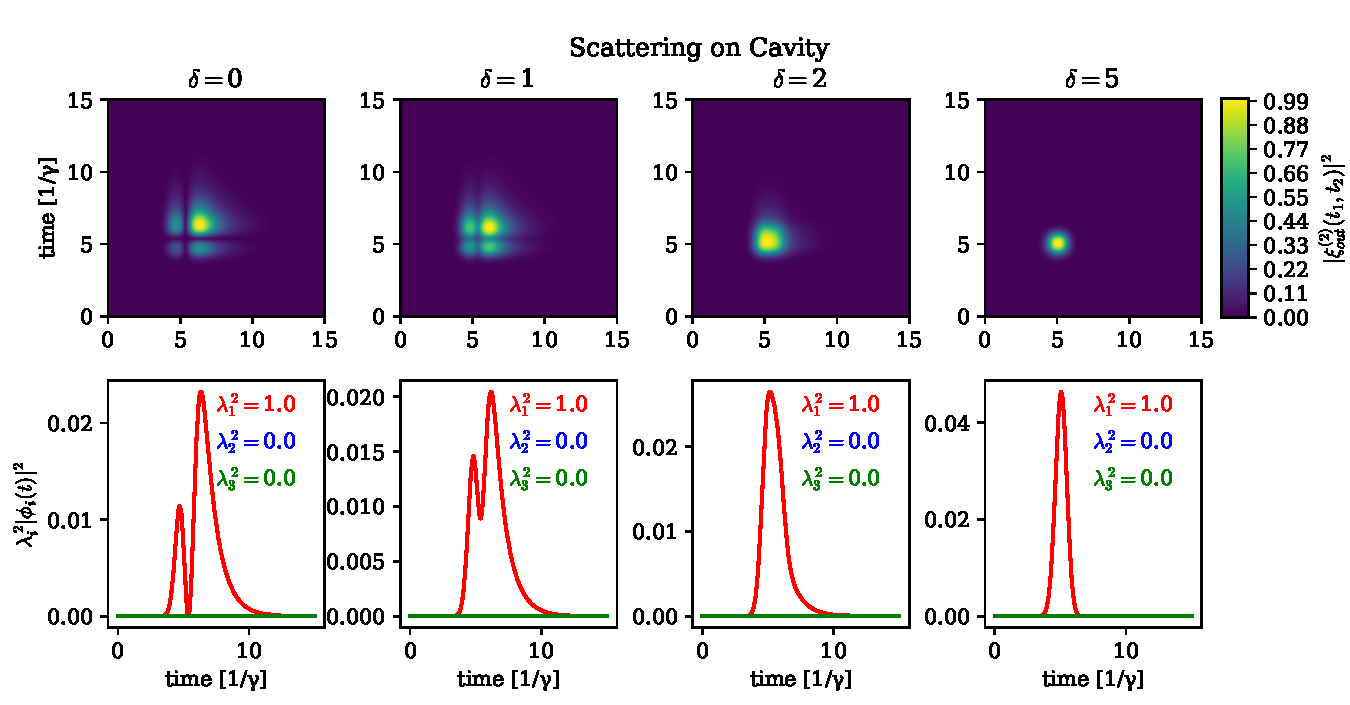
\includegraphics[width = 0.94\linewidth]{figures/twophoton_cavity_detuning.pdf}
    \caption{Scattering of a two-photon pulse on a single-sided cavity with a Gaussian product state $\ket{\psi}_{in} = \int dt \int dt' \xi_{in}^{(2)}(t,t') \ket{1_t}\ket{1_{t'}}$ where $ \xi_{in}^{(2)}(t,t') = \xi_{in}^{(1)}(t)\xi_{in}^{(1)}(t')$ with $\xi_{in}^{(1)}(t)$ given in eq.~\eqref{eq:gaussian} for different detunings $\delta$. Upper panels: The scattered two-photon state wavefunction $\xi_{out}^{(2)}(t,t')$ from the state $\ket{\psi}_{out} = \int dt \int dt' \xi_{out}^{(2)}(t,t') \ket{1_t}\ket{1_{t'}}$. All contour plots are normalized so that the largest value is unity. Lower panels: SVD (see eq.~\eqref{eq:SVD}) composition of the scattered two-photon state $\xi_{out}^{(2)}(t,t')$ with the three largest singular value functions shown. Noticeably only one SVD is relevant and the cavity thus also outputs a product state.} 
    \label{fig:twophoton_detuning}
\end{figure}



\begin{figure}
    \centering
    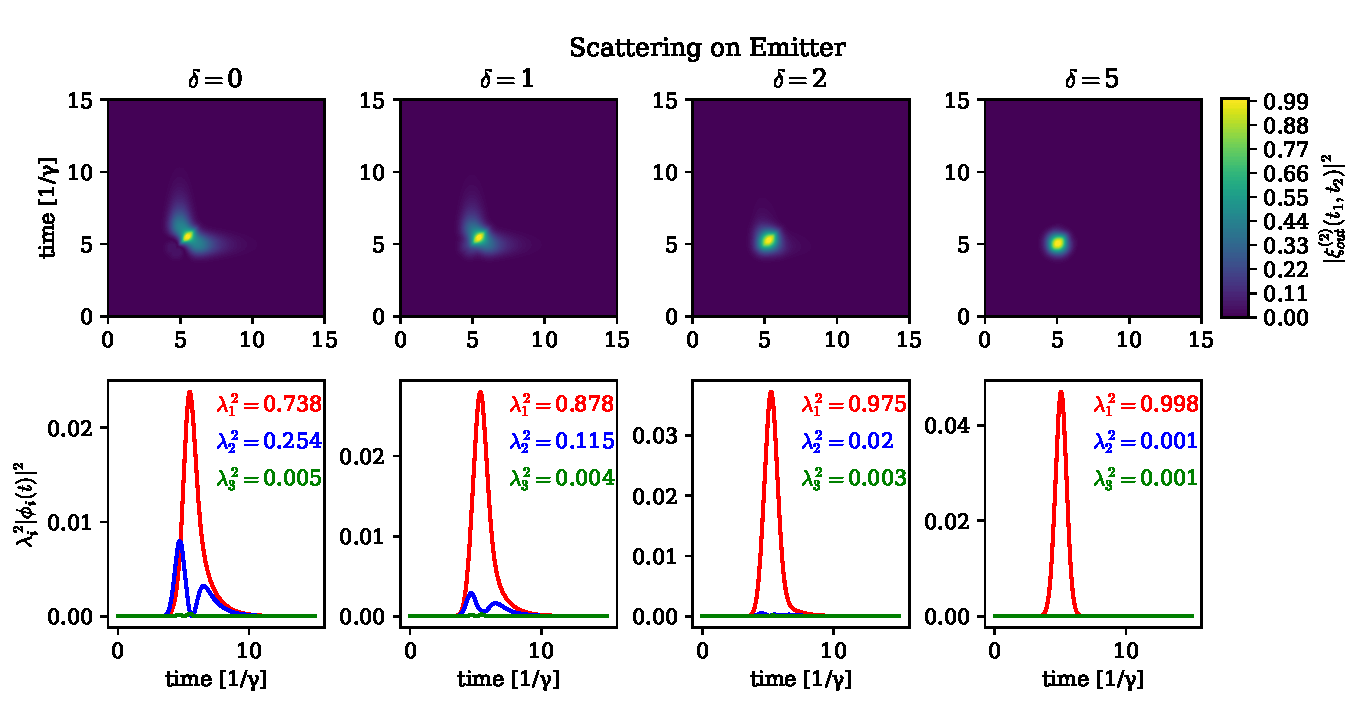
\includegraphics[width = 0.94\linewidth]{figures/twophoton_emitter_detuning.pdf}
    \caption{Same as Fig.~\ref{fig:twophoton_detuning} but scattering on a two-level system. The nonlinearity of the two-level-system gives an entangled two-photon state that can not be decomposed into a single function, which is seen in the SVD. }
    \label{fig:twophoton_emitter_detuning}
\end{figure}